\chapter{Software. Arquitectura e Implementación}
    \label{chap:five}
    
\section{Arquitectura e Implementación.}
\acrshort{murat} es un sistema software basado en una arquitectura multiagente que se ha implementado usando el lenguaje de programación \Gls{java}. Además, se han utilizado las siguientes librerías externas:
\begin{itemize}
    \item \textbf{JADE}: es una plataforma de código abierto el desarrollo de aplicaciones basadas en agentes. Simplifica la implementación de sistemas multiagente a través de un middle-ware que cumple con las especificaciones de la FIPA. \cite{jade}
    \item \textbf{Apache Commons \acrshort{csv}}: es una librería para trabajar con archivos de tipo \acrshort{csv}, tanto con operaciones de lectura como con operaciones de escritura.
    \item \textbf{Eclipse Source Minimal-\acrshort{json}}: es una librería de poco peso y eficiente que ofrece una \acrshort{api} completa para trabajar con archivos de tipo \acrshort{json}. 
\end{itemize}

El software está desarrollado siguiendo la estructura de paquetes estándar de los proyectos \Gls{java}. Existe un paquete genérico \lstinline{es.ugr.murat} que contiene a la clase principal del programa \lstinline{MURAT.java} y al resto de paquetes del mismo:
\begin{itemize}
    \item Clase \lstinline{MURAT.java}: es la clase principal la cual contiene la función \lstinline{main}. Se encarga de comenzar la simulación.
    \item Paquete \lstinline{agent}: contiene las clases agente del sistema:
    \begin{itemize}
        \item \lstinline{MURATBaseAgent.java}.
        \item \lstinline{TrafficLightAgent.java}
        \item \lstinline{CrossroadAgent.java}
        \item \lstinline{CityAgent.java}
    \end{itemize}
    \item Paquete \lstinline{appboot}: contiene la clase que se encarga de establecer la conexión con \acrshort{jade}:  
    \begin{itemize}
        \item \lstinline{JADEBoot.java}: clase encarga de establecer la conexión entre \acrshort{murat} y la plataforma \acrshort{jade}.
    \end{itemize}
    \item Paquete \lstinline{constant}: contiene las clases de constantes del sistema:
    \begin{itemize}
        \item \lstinline{ActionConstant.java}: clase representando las acciones que pueden realizar los agentes.
        \item \lstinline{CityConfigurationConstant.java}: clase representando las constantes usadas en la configuración de la ciudad (CityConfigurationModel).
        \item \lstinline{CityConstant.java}: clase representando las constantes del agente \textit{Ciudad} (\lstinline{CityAgent.java}).
        \item \lstinline{CommonConstant.java}: clase representando las constantes comunes.
        \item \lstinline{CrossroadConstant.java}: clase representando las constantes del agente \textit{Cruce} (\lstinline{CrossroadAgent.java}).
        \item \lstinline{JADEBootConstant.java}: clase representando las constantes utilizadas por la plataforma de agentes JADE.
        \item \lstinline{MessageConstant.java}: clase representando las constantes utilizadas por los agentes para el paso de mensajes.
        \item \lstinline{SimulationConstant.java}: clase representando las constantes de la clase \lstinline{Simulation.java}.
        \item \lstinline{TimeConstant.java}: clase representando los factores de conversión de unidades de tiempo.
        \item \lstinline{TrafficLightConstant.java}: clase representando las constantes del agente \textit{Semáforo} (\lstinline{TrafficLightAgent.java}).
    \end{itemize}
    \item Paquete \lstinline{helper}: contiene una clase auxiliar con algunas utilidades.
    \begin{itemize}
        \item \lstinline{Helper.java}: encapsula métodos de clase auxiliares para obtener tanto el origen como el destino de un tramo de cruce.
    \end{itemize}
    \item Paquete \lstinline{model}: contiene las clases modelo de las diferentes entidades que conforman el sistema.
    \begin{itemize}
        \item \lstinline{CityConfigurationModel.java}: clase representando el modelo de la configuración de la ciudad/escenario/simulación.
        \item \lstinline{CityModel.java}: clase representando el modelo de la ciudad.
        \item \lstinline{ConfigurationCrossroadInitialStateModel.java}: clase representando el modelo del estado inicial de un cruce.
        \item \lstinline{CrossroadModel.java}: clase representando el modelo de un cruce.
        \item \lstinline{CrossroadStretchModel.java}: clase representando el modelo de un tramo de cruce. Es un router que indica en qué cruce (Crossroad) se va desde qué calle (RoadStretchOrigin) hasta qué otra calle (RoadStretchDestination).
        \item \lstinline{RoadStretchModel.java}: clase representando el modelo de un tramo de calle.
        \item \lstinline{StateModel.java}: clase representando el modelo de un estado.
        \item \lstinline{TrafficLightModel.java}: clase representando el modelo de un semáforo.
    \end{itemize}
    \item Paquete \lstinline{simulation}: contiene la clase encargada de gestionar la obtención de información para la simulación, la creación de los agentes y la consulta de información necesaria por parte de los mismos.
    \begin{itemize}
        \item \lstinline{Simulation.java}: clase representando a una simulación, encargada de obtener todos los datos, lanzar los agentes y proveer a estos las funciones necesarias para la obtención de los datos que requieran.
    \end{itemize}
    \item Paquete \lstinline{util}: contiene una clase encargada de registrar mensajes.
    \begin{itemize}
        \item \lstinline{Logger.java}: clase encargada de registrar información de distinto tipo sobre la ejecución del programa.
    \end{itemize}
\end{itemize}

\newpage
\begin{figure}[H]
    \centering
    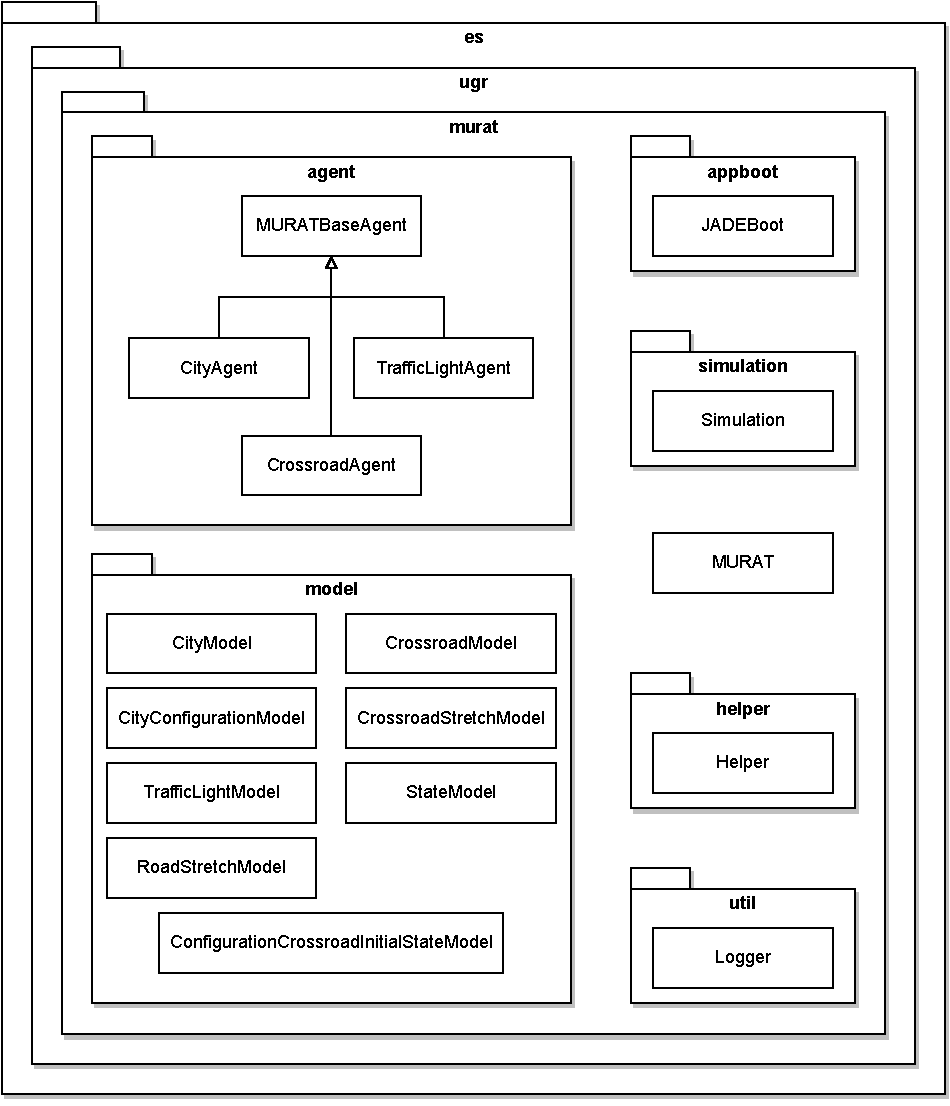
\includegraphics[width=1\linewidth]{text/image/DPaq.pdf}
    \caption{Diagrama de paquetes}
    \label{fig:diagrama_paquetes}
\end{figure}

La clase \lstinline{MURAT.java} únicamente tiene en su método \lstinline{main} la sentencia \lstinline{Simulation.start()}. Esta llamada al método de clase \lstinline{start()} de la clase \lstinline{Simulation.java} instancia el único objeto de esta clase que puede existir en la ejecución.


En primer lugar, la clase \lstinline{Simulation.java} muestra los paneles para la selección de la ciudad, el escenario y la política de tiempos a aplicar. Tras esto, carga toda la información del archivo \acrshort{json} correspondiente y construye las estructuras de datos necesarias. 
\begin{figure}[H]
    \centering
    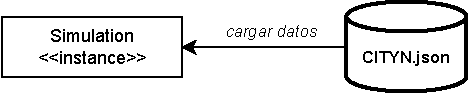
\includegraphics[width=0.8\linewidth]{text/image/D-Carga_de_datos.pdf}
    \caption{Diagrama de carga de datos para la simulación}
    \label{fig:diagrama_carga_datos}
\end{figure}

Más tarde, instancia un objeto de la clase \lstinline{JADEBoot.java}, el cual va a materializar la conexión con la plataforma \acrshort{jade}. A través de este objeto, usando el método \lstinline{launchAgent(String name,  Class<?> clazz)}, se lanzan todos los agentes del sistema.
\begin{figure}[H]
    \centering
    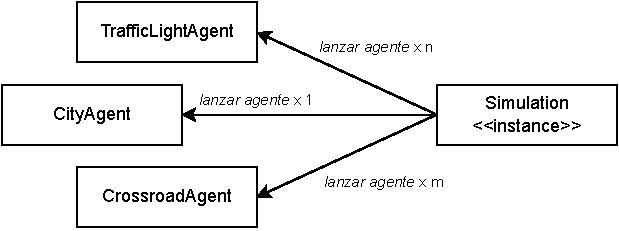
\includegraphics[width=1\linewidth]{text/image/D-Lanzamiento_de_agentes.pdf}
    \caption{Diagrama de lanzamiento de agentes}
    \label{fig:diagrama_lanzamiento_agentes}
\end{figure}

En este punto, empieza el ciclo de vida de los agentes. La clase \newline\lstinline{MURATBaseAgent.java}, clase padre de las clases de los agentes, extiende el comportamiento de la clase \lstinline{Agent.java} de \acrshort{jade}.La clase \lstinline{MURATBaseAgent.java}, común a todos los agentes, implementa un comportamiento por defecto que se basa en repetir una acción mientras no se haya indicado la salida (finalización) del agente. Este comportamiento se establece por defecto cuando se hace el setup del agente en el método \lstinline{setup()}. La acción a repetir se debe definir (implementar) sobrescribiendo el método \lstinline{execute()} de \lstinline{MURATBaseAgent.java}. Además del ya mencionado método, esta clase implementa otros métodos como: \lstinline{takeDown()}, para finalizar el agente; \lstinline{buildMessage(...)}, para construir un \acrshort{acl}Message; \lstinline{sendACLMessage(...)}, para enviar un \acrshort{acl}Message; y \lstinline{receiveACLMessage(...)}, para recibir un \acrshort{acl}Message.

El primer estado que comparten todos los agentes, como ya se ha explicado anteriormente, es el estado \textbf{\textit{Cargar datos}}. En este estado, cada uno de los agentes pide información al objeto {simulation}, a través de la interfaz que provee su clase, es decir, invocando a alguno de los getters existentes \lstinline{Simulation.simulation.get...()}.
\begin{figure}[H]
    \centering
    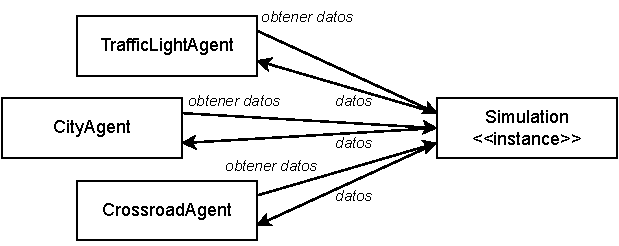
\includegraphics[width=1\linewidth]{text/image/D-Carga_de_datos S-As.pdf}
    \caption{Diagrama de carga de datos para los agentes}
    \label{fig:diagrama_carga_datos_agentes}
\end{figure}

A partir de este momento, los agentes ejecutan acciones en función de sus estados, tal y como se ha explicado en la sección \ref{section:sociedad_de_agentes}.

Un punto interesante a explicar es la adición de tráfico al sistema. Para cada instante de la simulación, se ejecuta el método \lstinline{addTraffic()} de la clase \lstinline{CrossroadAgent.java}. Cada agente \textit{Cruce} añade el tráfico correspondiente a cada tramo de calle de entrada al sistema (tramo de calle que no posee cruce de origen y cuyo cruce de destino es el propio cruce que añade los vehículos). En función de los ratios de entrada de vehículos al sistema, se calcula tanto el valor de vehículos por segundo que pueden entrar al tramo de calle como el valor de segundos que tarda un vehículo en poder entrar al tramo de calle. Estos cálculos se ven modificados en función del \textit{factor pico} \lstinline{PEAK_FACTOR} en caso de estar en alguno de los modos pico y en alguna de las horas pico. A partir de el valor definitivo de estas variables, se evalúa si por cada segundo entran uno o más vehículos o entra un vehículo cada varios segundos. En función de lo anterior, se añaden tantos vehículos como correspondan en cada segundo. Como anteriormente se ha comentado, existen tres modos de adición de tráfico al sistema:
\begin{itemize}
    \item \textbf{Lineal} (\textit{LINEAR}): durante toda la simulación entra al sistema de tráfico la misma cantidad de vehículos. La gráfica de adición de vehículos es una función lineal.
    \item \textbf{Pico único} (\textit{SINGLE PEAK}): durante toda la simulación entra al sistema de tráfico la misma cantidad de vehículos a excepción de en un intervalo pico determinado, donde entra una cantidad mucho mayor. La gráfica de adición de vehículos es una función lineal que tiene un intervalo en el que la pendiente de la función aumenta con respecto a su valor hasta el inicio de ese intervalo. Ese intervalo se corresponde con la duración de la hora pico, representada en el eje X (tiempo). 
    \item \textbf{Pico doble} (\textit{DOUBLE PEAK}): durante toda la simulación entra al sistema de tráfico la misma cantidad de vehículos a excepción de en dos intervalos pico determinados, donde entran unas cantidades mucho mayores. La gráfica de adición de vehículos es una función lineal que tiene dos intervalos en los que la pendiente de la función aumenta con respecto a su valor hasta el inicio de esos intervalos. Esos intervalos se corresponden con la duración de las horas pico, representadas en el eje X (tiempo). 
\end{itemize}


Para finalizar con estos apartados dedicados a la implementación del sistema, se va a explicar el algoritmo de optimización de tiempos de estados de los semáforos utilizado. El método que aplica la optimización de los tiempos se denomina \lstinline{optimizeStateTimes(...)} y forma parte de la clase \lstinline{CrossroadAgent.java}. Este método se ejecuta cada segundo de la simulación. Se realizan los siguientes pasos:
\begin{enumerate}
    \item Se obtienen los tramos de calle de entrada congestionados y sus puntuaciones de congestión asociadas. Esto se realiza usando el método \lstinline{getCongestedRoadStretchesIn()}. Se considera que un tramo de calle está saturado cuando su porcentaje de ocupación es mayor que el umbral de saturación, \lstinline{SATURATION_THRESHOLD}. Si un tramo de calle está saturado, se añade al mapa de tramos de calle de entrada congestionados y se le asocia una puntuación de congestión, calculada en base al número de vehículos y el porcentaje de ocupación, multiplicando cada uno de estos valores por sus pesos, \lstinline{VEHICLE_WEIGHT} y \lstinline{OCCUPATION_WEIGHT}, y sumándolos.
    \item Se evalúa si existe algún tramo de calle de entrada con congestión. 
        \begin{itemize}
            \item Si no existe no se continúa. Se vuelve a repetir el proceso en la siguiente iteración.
            \item Si existe se continúa.
        \end{itemize}
    \item Se analiza si existe algún estado del cruce que beneficie la salida de tráfico de los tramos de calle, es decir, algún estado del cruce que habilite tramos de cruce cuyos tramos de calle de origen sean el mayor número de entre los congestionados.
    \begin{itemize}
        \item Se obtienen para cada estado los tramos de calle de entrada congestionados que habilita y sus puntuaciones de congestión asociadas.
        \item Se obtienen los candidatos a ser el mejor estado, en función de los tramos de calle origen saturados cuyos tramos de cruce asociados son habilitados.
        \item Se obtienen los candidatos a ser el peor estado, en función de los tramos de calle origen saturados cuyos tramos de cruce asociados son habilitados.
    \end{itemize}
    \item Se elige el mejor estado entre los candidatos, es decir, el estado que habilite tramos de cruce tales que la suma de las puntuaciones de congestión de sus tramos de calle de origen sea la mayor.
    \item Se elige el peor estado entre los candidatos, es decir, el estado que habilite menos tramos de cruce o habilitándolos tales que la suma de las puntuaciones de congestión de sus tramos de calle de origen sea la menor.
    \item Se ajustan los tiempos. Se aumenta el tiempo del mejor estado y se resta la misma cantidad de tiempo que se ha aumentado al mejor estado al peor estado.

\end{enumerate}

\newpage
\section{¿Cómo realizar una simulación? Pasos para ejecutar el software}
En primer lugar, es necesario situarse en el directorio \lstinline{es.ugr.murat}. Estando en el directorio mencionado y teniendo una versión de \Gls{java} 17 instalada en el sistema y accesible a través de la terminal que se use, es decir, teniendo el directorio \lstinline{bin} de la versión de \Gls{java} en la variable de entorno \lstinline{PATH}, es necesario hacer lo siguiente.
\begin{enumerate}
    \item \textbf{Arrancar la plataforma de agentes} \acrshort{jade} con la siguiente orden:\newline 
    \lstinline{java -cp lib\jade.jar jade.Boot -gui -host localhost}
\end{enumerate}
\begin{figure}[H]
    \centering
    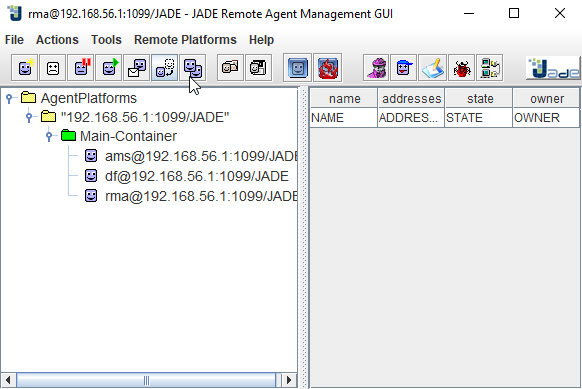
\includegraphics[width=1\linewidth]{text/image/Ejec_JADEGUI.png}
    \caption{GUI de JADE que aparece tras arrancar la plataforma}
    \label{fig:ejec_jadegui}
\end{figure}

\begin{enumerate}
    \setcounter{enumi}{1}
    \item \textbf{Iniciar el sistema} \acrshort{murat}:
    \begin{itemize}
        \item Importar el proyecto de IntelliJ.
        \item Seleccionar la configuración de Run/Debug correspondiente a \acrshort{murat}.
        \item Pulsar en el botón de play \textit{'Run' \acrshort{murat}}.
    \end{itemize}
\end{enumerate}

Al iniciar el sistema \acrshort{murat} aparece un selector de ciudad.
\begin{figure}[H]
    \centering
    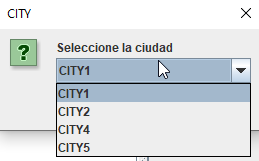
\includegraphics[width=0.5\linewidth]{text/image/Ejec_CITY.png}
    \caption{Selección de la ciudad}
    \label{fig:ejec_city}
\end{figure}

Más tarde, una vez seleccionada la ciudad, aparece un selector de configuración que muestra las configuraciones posibles para la ciudad seleccionada.
\begin{figure}[H]
    \centering
    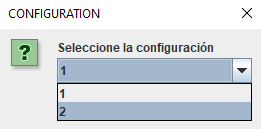
\includegraphics[width=0.5\linewidth]{text/image/Ejec_CONFIGURATION.png}
    \caption{Selección de la configuración}
    \label{fig:ejec_configuracion}
\end{figure}

Tras haber elegido ciudad y configuración, aparece un selector para elegir la política de tiempos que se quiere aplicar en la simulación.
\begin{figure}[H]
    \centering
    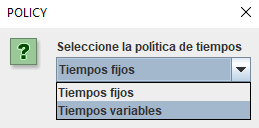
\includegraphics[width=0.5\linewidth]{text/image/Ejec_POLICY.png}
    \caption{Selección de la política de tiempos}
    \label{fig:ejec_policy}
\end{figure}

Una vez elegidas ciudad, configuración y política de tiempos comienza la simulación. La simulación no se completa de forma inmediata, por lo tanto, hay que esperar unos minutos. Se puede observar en los logs del programa todo lo que está sucediendo en cada momento. Cuando la simulación finaliza se genera un archivo de tipo \acrshort{csv} en el directorio \lstinline{resources/data/results} con los resultados de la simulación.